




\subsection{Software}

\begin{frame}[allowframebreaks]{Software}{Für Desktop}
 
\note{Für Informatiker ist Linux geeignet, weil deren Software gut auf Linux läuft\\}
\hspace{1cm}

\begin{description}[style=nextline]
 
 \item [Browser] {\bf Firefox}, Chromium, Vivaldi, Opera, Tor
  \item [\small statt] Edge, Explorer
 \item [Office] {\bf LibreOffice}, Kile (\LaTeX), \TeX maker
  \item [\small statt] MS Office (365)
 \item [Email Clients] {\bf Thunderbird}, Icedove, Evolution 
  \item [\small statt] Outlook
\pagebreak 
 \item [IDEs] {\bf Eclipse}, IntelliJ, NetBeans, Atom, VI(M)
  \item [\small statt] Visual Studio
 \item [Medien]{\bf VLC}, Audacity, Rythmbox, Totem
\item [\small statt] \textit{altem} Windows Media Player
 \item [Grafik] {\bf GIMP}, Blender,  Inkscape
  \item [\small statt] Photoshop, Illustrator, etc.
 \item [alles] DAS TERMINAL 

\end{description}
 \end{frame}


 \begin{frame}{Software}{Wie bekomme ich die?}

  \begin{columns}
  \begin{column}{0.3\textwidth}
 \begin{figure}
 
\includegraphics[height=0.5\textheight]{resources/garbage-296550_1280.png}
  %https://pixabay.com/en/garbage-electronics-trash-rubbish-296550/
 \end{figure}
\end{column}
\begin{column}{0.6\textwidth}
 \begin{center}
   \textbf{\large{ Paketverwaltung}}
 \end{center}
\note{wegen seiner genialität inzwischen bei Apple, Google Play, Appstore.., Microsoft\\}
%TODO: pakete sind komplette Konfigurationen, die die gesamte Installation und Einrichtung mit einem Befehl/ Klick zu installieren.
  \begin{itemize}
   \item Einfache Installation \note{globle liste der Software\\}
   \begin{itemize}
    \item {\normalsize 1 Klick / Befehl}
    \item {\normalsize Große Auswahl aus Liste}
    \item {\normalsize Fertige Konfigurationen} \note{ uuund von wem?...  Das machen die Distros, den es gibt verschiedne Repos.. natürlich..\\}
    \item {\normalsize Automatische Abhängikeiten} \note { Erleichtert die Installation von Software, weil alle nötigen Dinge notiert sind}
   \end{itemize}

   \item Sicher \note{Auch hier muss man natürlich vertrauen, aber bei Linux muss man eben seltener ausweichen\\}
   \item Kein Balast \note{damit euer Rechner nicht im Müll versinkt\\}
  \end{itemize}
  \end{column}
  \end{columns}
 \end{frame}

 



\subsection{Distros}
\begin{frame}{Distributionen?}{Was ist das?}
\begin{columns}
\begin{column}{0.45\textwidth}

Kümmern sich um: \note{passende Software zusammenstellen\\} \note{Fehler beheben, Änderungen vorhnehmen (mint, ubuntu)\\}
\begin{itemize}
 \item Software $\longrightarrow$ Pakete
 \item Änderungen/Patches
 \item Hilfe/Support \note{und mit Support kann man Geld verdienen\\}
\end{itemize}
 Betrieben von: \note{kernel- nicht alleine nutzbar\\}
\begin{itemize}
 \item Community
 \item Firmen
\end{itemize}
 \end{column}
\begin{column}{0.4\textwidth}
 \begin{figure}
 
\includegraphics[height=0.5\textheight]{resources/movers-24402_640.png}
 %https://pixabay.com/en/movers-moving-carry-lift-walk-24402/
 \end{figure}
\end{column}
\end{columns}
 \end{frame}



\begin{frame}{Distributionen!}{Zum Beispiel:}
\note{Mint, OpenSuse, ubuntu, Fedora\\}
\note{alle direkt benutzbar}
\begin{columns}
\begin{column}{0.5\textwidth}
\begin{figure}

\includegraphics[width=0.9\textwidth]{resources/640px-Linux_Mint_logo_and_wordmark}
%https://de.wikipedia.org/wiki/Linux_Mint#/media/File:Linux_Mint_logo_and_wordmark.svg
\end{figure}

\begin{figure}

\includegraphics[width=0.8\textwidth]{resources/640px-OpenSUSE_Logo}
%https://de.wikipedia.org/wiki/OpenSUSE#/media/File:OpenSUSE_Logo.svg
\end{figure}

 \end{column}
\begin{column}{0.5\textwidth}

\begin{figure}

\includegraphics[width=0.9\textwidth]{resources/640px-Ubuntu_logo}
%https://de.wikipedia.org/wiki/Ubuntu#/media/File:Ubuntu_logo.svg
\end{figure}

\begin{figure}

\includegraphics[width=0.9\textwidth]{resources/640px-Fedora_logo_and_wordmark}
%https://de.wikipedia.org/wiki/Fedora_%28Linux-Distribution%29#/media/File:Fedora_logo_and_wordmark.svg
\end{figure}

\end{column}
\end{columns}
\end{frame}

\subsection{Oberflächen}
\begin{frame}{Oberflächen}{Gnome}
\note{komplett tauschbare Oberflächen/DEs}
\note{Gnome3\\}
\begin{figure}
 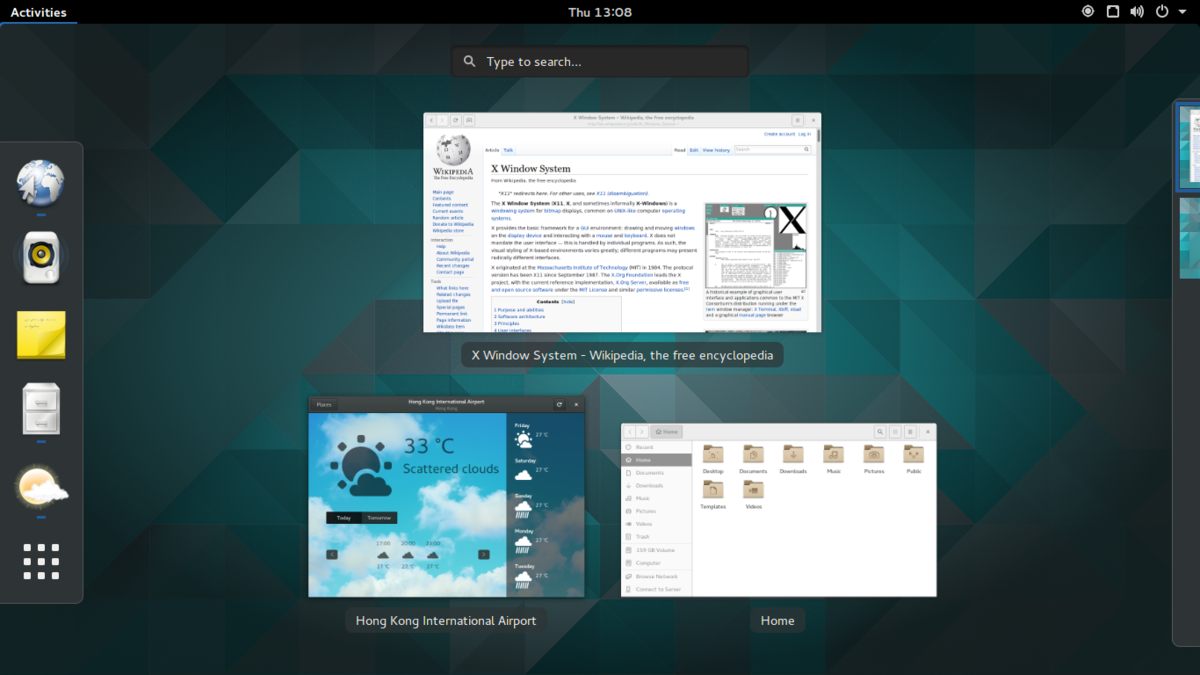
\includegraphics[height=0.6\textheight]{resources/1200px-GNOME_Shell.png}
 %https://de.wikipedia.org/wiki/Gnome-Shell#/media/File:GNOME_Shell.png
 \end{figure}

\end{frame}

\begin{frame}{Oberflächen}{KDE}

\note{KDE/Plasma\\}
\begin{figure}
 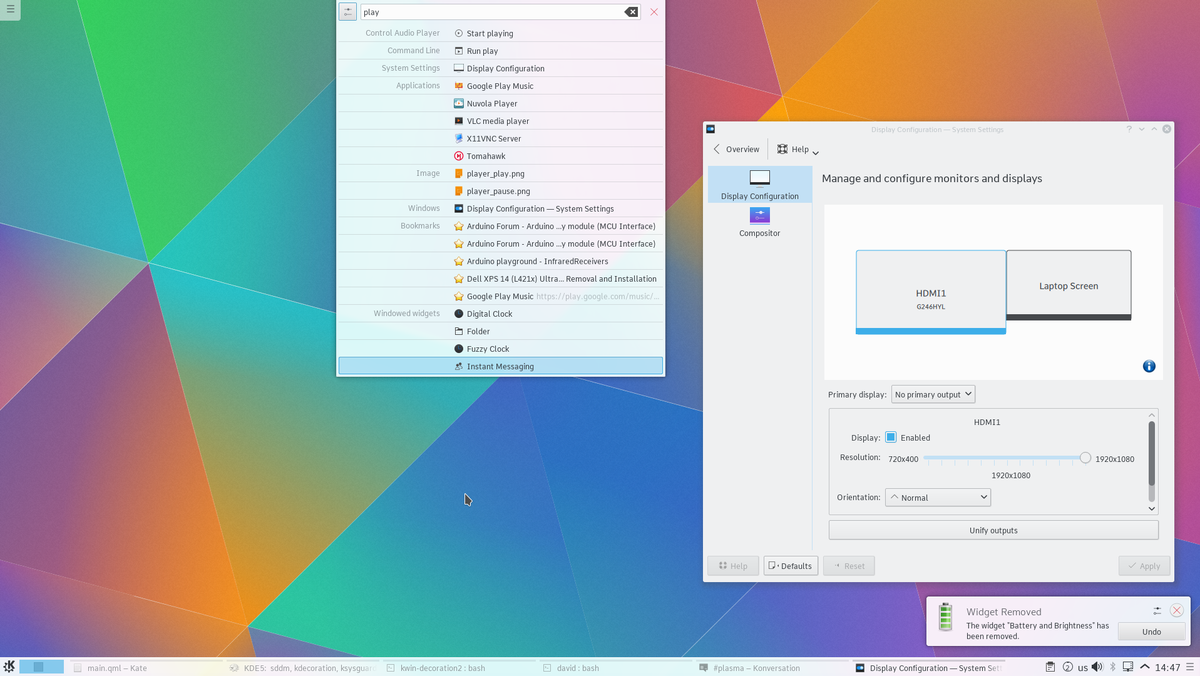
\includegraphics[height=0.6\textheight]{resources/1200px-Kscreen-krunner.png}
 %https://en.wikipedia.org/wiki/KDE_Plasma_5#/media/File:Kscreen-krunner.png
 \end{figure}


\end{frame}

\begin{frame}{Oberflächen}{Cinnamon}
\note{Cinnamon/Mint\\}
\begin{figure}
 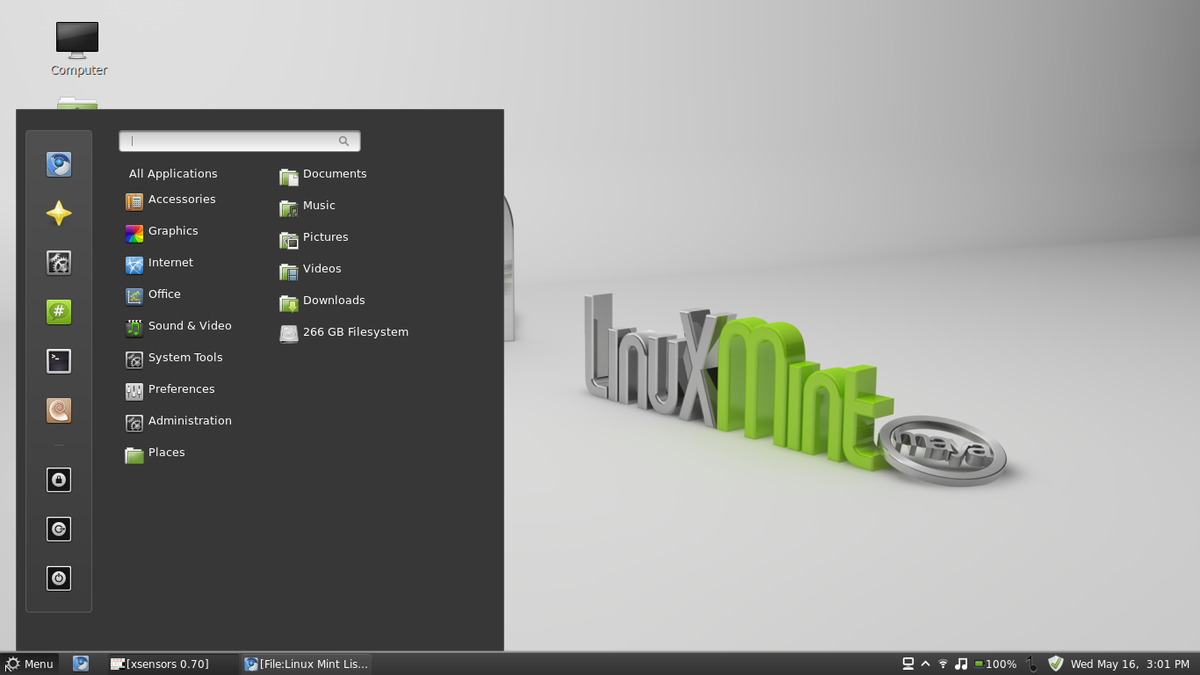
\includegraphics[height=0.6\textheight]{resources/1200px-Linux_Mint.png}
 %https://de.wikipedia.org/wiki/Cinnamon_(Desktop-Umgebung)#/media/File:Linux_Mint_13_RC.png
 \end{figure}


\end{frame}


 





